\chapter{Enols, Enolates and the Aldol Reaction}\label{ch:b2:enolates-aldol}

Every time a cell breaks down glucose, an enzyme cuts a six-carbon sugar
phosphate into two three-carbon pieces: an \omterm{def:b2:enolates-aldol:aldol}{aldol} reaction run backwards. Run
forwards, the same reaction joins two carbonyl compounds into one, and it is
the chemist's most used way of making carbon--carbon bonds. It rests on a
property that the previous chapters only touched: the hydrogen atoms next to a
carbonyl group are acidic, and removing one turns the carbon beside the
carbonyl into a nucleophile.

\begin{recall}
The Year 1 volume: $\mathrm pK_a$ and the predominant reaction, carbanions, kinetic and
thermodynamic control, \omterm{def:b2:amines:nucleophilic-addition}{nucleophilic additions} to carbonyls, E1 and E2 eliminations, the hydration of
alkynes (an \omterm{def:b2:enolates-aldol:tautomerism}{enol} rearranging). \Cref{ch:b2:frontier-orbitals}: \omterm{def:b2:frontier-orbitals:ambident}{ambident nucleophiles}.
\Cref{ch:b2:acyl-substitution}: esters and acyl substitution.
\end{recall}

\section{Keto--enol tautomerism}

\begin{definition}[Tautomerism]\label{def:b2:enolates-aldol:tautomerism}
\emph{Tautomers}\index{tautomers} are isomers that interconvert by moving a hydrogen and a double
bond. In \emph{keto--enol tautomerism}\index{keto--enol tautomerism}, a carbonyl compound with a
hydrogen on the carbon next to the carbonyl (the keto form) is in equilibrium with its
\emph{enol}\index{enol}, an alcohol carried by a \ce{C=C} double bond.
\end{definition}

\begin{omfigure}
\setchemfig{atom sep=2em}
\schemestart
\chemfig{H_3C-C(=[2]O)-CH_3}
\arrow{<=>[\ce{H+} or \ce{HO-}][catalysis]}[,2.2]
\chemfig{H_3C-C(-[2]OH)=CH_2}
\schemestop
\par\vspace{6pt}

{\small Propanone and its \omterm{def:b2:enolates-aldol:tautomerism}{enol}, prop-1-en-2-ol. Acid (protonation of the carbonyl oxygen, then loss
of an $\alpha$ hydrogen) or base (removal of an $\alpha$ hydrogen, then protonation of the oxygen)
catalyses the interconversion; the equilibrium lies far on the side of the keto form.}
\end{omfigure}

\begin{proposition}[Enol content]\label{prop:b2:enolates-aldol:enol-content}
Simple aldehydes and ketones contain only traces of \omterm{def:b2:enolates-aldol:tautomerism}{enol}; 1,3-dicarbonyl compounds such as
pentane-2,4-dione contain a large proportion of it.
\end{proposition}

\begin{proof}[Argument]
A \ce{C=O} bond is stronger than a \ce{C=C} bond by more than an \ce{O-H} bond is weaker than a \ce{C-H}
bond: the keto form is favoured. In a 1,3-dicarbonyl compound, the \omterm{def:b2:enolates-aldol:tautomerism}{enol} double bond is conjugated
with the second carbonyl group, and the \omterm{def:b2:enolates-aldol:tautomerism}{enol} \ce{OH} forms an internal hydrogen bond with its oxygen
in a six-membered ring: both stabilise the \omterm{def:b2:enolates-aldol:tautomerism}{enol} enough to make it a major form.
\end{proof}

Because the \omterm{def:b2:enolates-aldol:tautomerism}{enol} is planar at its \ce{C=C}, a stereocentre at the $\alpha$ carbon is lost each time
the \omterm{def:b2:enolates-aldol:tautomerism}{enol} forms: an optically active ketone with a stereocentre next to its carbonyl racemises in acid
or base.

\section{Enolates}

\begin{definition}[Enolates]\label{def:b2:enolates-aldol:enolate}
The \emph{$\alpha$ carbon}\index{alpha carbon@$\alpha$ carbon} of a carbonyl compound is the carbon
bound to the carbonyl carbon; its hydrogens are \emph{$\alpha$ hydrogens}\index{alpha hydrogen@$\alpha$ hydrogen}.
Removing one gives an \emph{enolate ion}\index{enolate ion}, whose
negative charge is shared between the $\alpha$ carbon and the oxygen.
\end{definition}

\begin{proposition}[Acidity of $\alpha$ hydrogens]\label{prop:b2:enolates-aldol:alpha-acidity}
$\alpha$ hydrogens are far more acidic than ordinary \ce{C-H} bonds because the \omterm{def:b2:enolates-aldol:enolate}{enolate} is stabilised
by resonance; a hydrogen between two carbonyl groups is acidic enough to be removed by an alkoxide or
even hydroxide.
\end{proposition}

\begin{proof}[Argument]
In the \omterm{def:b2:enolates-aldol:enolate}{enolate} the negative charge sits partly on the electronegative oxygen; a second carbonyl on
the other side delocalises it over two oxygens. Measured in water, pentane-2,4-dione has $\mathrm pK_a =
9.0$ and ethyl 3-oxobutanoate 10.7, comparable with nitromethane (10.2), whose anion is stabilised
by the nitro group in the same way; a simple ketone, with only one carbonyl, is far weaker --- too weak
for its acidity to be measured directly in water.
% ledger: pka:acac, pka:acetoacetate, pka:nitromethane
\end{proof}

\begin{omfigure}
\setchemfig{atom sep=2em}
\schemestart
\chemfig{H_3C-C(=[2]O)-\chemabove{C}{\scriptstyle -}H_2}
\arrow{<->}
\chemfig{H_3C-C(-[2]\chemabove{O}{\scriptstyle -})=CH_2}
\schemestop
\par\vspace{6pt}

{\small The two resonance structures of the \omterm{def:b2:enolates-aldol:enolate}{enolate} of propanone. The negative charge is shared by
the $\alpha$ carbon and the oxygen: the \omterm{def:b2:enolates-aldol:enolate}{enolate} is an \omterm{def:b2:frontier-orbitals:ambident}{ambident nucleophile}, reacting with most carbon
electrophiles at carbon.}
\end{omfigure}

\begin{definition}[Kinetic and thermodynamic enolates]\label{def:b2:enolates-aldol:kinetic-enolate}
For a ketone with two different $\alpha$ carbons, the \emph{kinetic enolate}\index{kinetic enolate}
is the one formed faster, by removal of a hydrogen from the less hindered, less substituted side; the
\emph{thermodynamic enolate}\index{thermodynamic enolate} is the more stable one, with the more
substituted double bond.
\end{definition}

\begin{proposition}[Choosing the enolate]\label{prop:b2:enolates-aldol:enolate-control}
A strong, bulky base used in full at low temperature (lithium diisopropylamide, LDA, at
\qty{-78}{\degreeCelsius}) forms the \omterm{def:b2:enolates-aldol:kinetic-enolate}{kinetic enolate} completely and irreversibly; a weaker base at room
temperature (an alkoxide in its alcohol) lets the \omterm{def:b2:enolates-aldol:enolate}{enolates} interconvert and gives mostly the
thermodynamic one.
\end{proposition}

\begin{proof}[Argument]
LDA ($\mathrm pK_a$ of diisopropylamine near 36, far above that of the ketone) deprotonates completely and
fast; at low temperature the \omterm{def:b2:enolates-aldol:enolate}{enolate} is not reprotonated, and the faster deprotonation, at the
accessible \ce{CH2} or \ce{CH3}, decides: kinetic control. An alkoxide removes the proton only partly,
the \omterm{def:b2:enolates-aldol:enolate}{enolates} and the ketone exchange protons continually, and the equilibrium mixture favours the
more substituted, more stable \omterm{def:b2:enolates-aldol:enolate}{enolate}: thermodynamic control (as in the Year 1 volume).
% ledger: ghs:LDA
\end{proof}

\section{Alkylating enolates}

\omterm{def:b2:enolates-aldol:enolate}{Enolates} attack primary halogenoalkanes by bimolecular substitution, forming a new \ce{C-C} bond at
the $\alpha$ carbon. With the very acidic $\alpha$ hydrogens of a 1,3-dicarbonyl compound, an alkoxide
suffices, and the extra carbonyl can be removed afterwards.

\begin{definition}[Decarboxylation]\label{def:b2:enolates-aldol:decarboxylation}
A \emph{decarboxylation}\index{decarboxylation} removes a carboxyl group as \ce{CO2}. In the
\emph{malonic ester synthesis}\index{malonic ester synthesis}, diethyl propanedioate is deprotonated,
alkylated, hydrolysed to the substituted propanedioic acid and decarboxylated by heating, giving a
carboxylic acid \ce{RCH2COOH}.
\end{definition}

\begin{proposition}[Easy decarboxylations]\label{prop:b2:enolates-aldol:decarboxylation}
$\beta$-keto acids and propanedioic acids lose \ce{CO2} on gentle heating; ordinary carboxylic acids
do not.
\end{proposition}

\begin{proof}[Argument]
The carbonyl two bonds away from the carboxyl group accepts the hydrogen of \ce{COOH} in a cyclic,
six-membered transition state while \ce{CO2} leaves: an \omterm{def:b2:enolates-aldol:tautomerism}{enol} forms directly, then tautomerises. Without
that carbonyl, the carbanion that loss of \ce{CO2} would leave behind has no stabilisation.
\end{proof}

\begin{definition}[Haloform reaction]\label{def:b2:enolates-aldol:haloform}
The \emph{haloform reaction}\index{haloform reaction} converts a methyl ketone \ce{RCOCH3}, with a
halogen and excess hydroxide, into a carboxylate \ce{RCOO-} and a haloform \ce{CHX3}.
\end{definition}

Each halogen introduced makes the remaining $\alpha$ hydrogens more acidic, so the methyl group is
trihalogenated; the \ce{CX3-} group is then a good enough leaving group to be expelled by hydroxide in an
acyl substitution. With iodine, the yellow precipitate of iodoform is a test for methyl ketones.

\section{The aldol reaction}

\begin{definition}[Aldol reactions]\label{def:b2:enolates-aldol:aldol}
In an \emph{aldol addition}\index{aldol addition} the \omterm{def:b2:enolates-aldol:enolate}{enolate} (or \omterm{def:b2:enolates-aldol:tautomerism}{enol}) of one carbonyl compound adds
to the carbonyl group of another, giving a $\beta$-hydroxy carbonyl compound, an
\emph{aldol}\index{aldol}. In an \emph{aldol condensation}\index{aldol condensation} the aldol loses
water, giving an $\alpha,\beta$-unsaturated carbonyl compound (an enone or enal).
\end{definition}

\begin{omfigure}
\setchemfig{atom sep=1.9em}
\schemestart
\chemfig{H_3C-CH=O} \+ \chemfig{^{-}CH_2-CH=O}
\arrow{->[addition]}
\chemfig{H_3C-CH(-[2]O^{-})-CH_2-CH=O}
\schemestop

\medskip
\schemestart
\arrow{->[\ce{H2O}][$-$ \ce{HO-}]}
\chemfig{H_3C-CH(-[2]OH)-CH_2-CH=O}
\arrow{->[heat, base][$-$ \ce{H2O}]}
\chemfig{H_3C-CH=CH-CH=O}
\schemestop
\par\vspace{6pt}

{\small The \omterm{def:b2:enolates-aldol:aldol}{aldol} reaction of ethanal. The \omterm{def:b2:enolates-aldol:enolate}{enolate} adds to a second molecule of ethanal; protonation
gives the \omterm{def:b2:enolates-aldol:aldol}{aldol}, 3-hydroxybutanal. On heating with base, an $\alpha$ hydrogen is removed and hydroxide
leaves from the $\beta$ carbon: but-2-enal, conjugated.}
\end{omfigure}

\begin{proposition}[Driving the aldol]\label{prop:b2:enolates-aldol:aldol-equilibrium}
The \omterm{def:b2:enolates-aldol:aldol}{aldol addition} is reversible; the dehydration, which forms a conjugated system, pulls the
reaction towards the condensation product.
\end{proposition}

\begin{proof}[Argument]
Two molecules give one, so the entropy of reaction is negative, and the new \ce{C-C} bond hardly
outweighs the lost \ce{C=O} $\pi$ bond: for many ketones $K$ is small. Removing the \omterm{def:b2:enolates-aldol:aldol}{aldol} by dehydration
keeps $Q < K$ for the addition; the conjugated enone formed is stabilised and, at high temperature,
the entropy gain of releasing water favours it further. The reverse reaction, the \omterm{def:b2:enolates-aldol:aldol}{retro-aldol}, is the
step by which the cell splits a six-carbon sugar.
\end{proof}

\begin{method}[Controlling a crossed aldol]\label{met:b2:enolates-aldol:crossed-aldol}
\begin{enumerate}
  \item Use one partner without $\alpha$ hydrogens (benzaldehyde, methanal): it can only be the
        electrophile.
  \item Or form the \omterm{def:b2:enolates-aldol:enolate}{enolate} of one partner completely first (LDA, \qty{-78}{\degreeCelsius}), then add
        the other.
  \item Or use a 1,3-dicarbonyl partner, far more acidic than the other.
  \item Prefer an aldehyde as electrophile: it is more reactive than a ketone.
\end{enumerate}
\end{method}

\begin{method}[Recognising an aldol product]\label{met:b2:enolates-aldol:aldol-recognition}
\begin{enumerate}
  \item Look for a \ce{C=O} with an \ce{OH} on the carbon two atoms away ($\beta$), or for a \ce{C=C}
        conjugated with a \ce{C=O}.
  \item Cut the bond between the $\alpha$ and $\beta$ carbons: the $\beta$ carbon was a carbonyl carbon (the
        electrophile), the $\alpha$ carbon the \omterm{def:b2:enolates-aldol:enolate}{enolate} carbon.
  \item Check that the two partners exist and that the \omterm{def:b2:enolates-aldol:enolate}{enolate} can be formed selectively.
\end{enumerate}
\end{method}

\section{The Claisen condensation}

\begin{definition}[Claisen condensation]\label{def:b2:enolates-aldol:claisen}
In a \emph{Claisen condensation}\index{Claisen condensation}, the \omterm{def:b2:enolates-aldol:enolate}{enolate} of an ester attacks the
carbonyl of another ester molecule in an acyl substitution, giving a \emph{$\beta$-keto ester}\index{beta-keto ester@$\beta$-keto ester}
and releasing an alkoxide. Its intramolecular version, the Dieckmann
cyclisation, gives a cyclic $\beta$-keto ester.
\end{definition}

\begin{proposition}[What drives the Claisen]\label{prop:b2:enolates-aldol:claisen-drive}
The \omterm{def:b2:enolates-aldol:claisen}{Claisen condensation} of ethyl ethanoate needs a full equivalent of sodium ethoxide: its equilibrium
is unfavourable, and it is driven by the deprotonation of the $\beta$-keto ester formed.
\end{proposition}

\begin{proof}
The condensation proper, \ce{2CH3COOEt <=> CH3COCH2COOEt + EtOH}, has a small equilibrium constant
$K_1$. The $\beta$-keto ester ($\mathrm pK_a = 10.7$) is then deprotonated by ethoxide (ethanol, 15.9):
$K_2 = 10^{15.9 - 10.7} = 10^{5.2}$. The overall reaction, condensation plus deprotonation, has
$K_1K_2$, large enough even for small $K_1$; the base is consumed and an acid work-up gives the neutral
$\beta$-keto ester. An ester with only one $\alpha$ hydrogen, whose product cannot be deprotonated, gives
little product.
% ledger: pka:acetoacetate, pka:ethanol
\end{proof}

\begin{history}[The aldol, 1872]
\begin{minipage}[t]{0.18\linewidth}
\vspace{0pt}
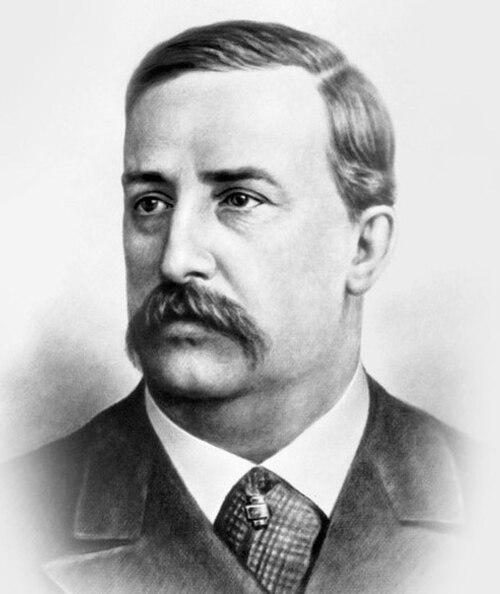
\includegraphics[width=\linewidth]{images/book3/borodin.jpg}
\end{minipage}\hspace{0.02\linewidth}%
\begin{minipage}[t]{0.18\linewidth}
\vspace{0pt}
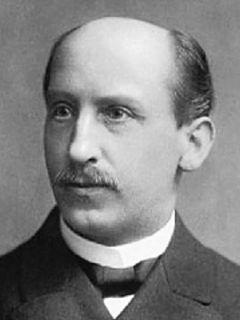
\includegraphics[width=\linewidth]{images/book3/claisen.jpg}
\end{minipage}\hfill
\begin{minipage}[t]{0.58\linewidth}
\vspace{0pt}
The \omterm{def:b2:enolates-aldol:aldol}{aldol} reaction was described in 1872 by Charles-Adolphe Wurtz and, independently, by Alexander
Borodin, a chemist in Saint Petersburg better known today as the composer of \textit{Prince Igor}.
Ludwig Claisen extended the condensations of carbonyl compounds to esters in 1887. (Portraits: Borodin,
unknown author, public domain; Claisen, by Veronica.villagrasa, CC BY-SA 4.0; Wikimedia Commons.)
\end{minipage}
\end{history}

\begin{safety}{\ghs[5mm]{GHS02}\,\ghs[5mm]{GHS05}\,\ghs[5mm]{GHS07}}
Sodium ethoxide and lithium diisopropylamide are corrosive and react with water; LDA solutions are
flammable and handled under inert gas. Benzaldehyde and propanone are harmful and flammable.
% ledger: ghs:NaOEt, ghs:LDA, ghs:benzaldehyde, ghs:acetone
\end{safety}

\section{Exercises}

\begin{exercise}[$\star$]\label{exo:b2:enolates-aldol:1}
Draw the \omterm{def:b2:enolates-aldol:tautomerism}{enol} \omterm{def:b2:enolates-aldol:tautomerism}{tautomers} of butanone and of cyclohexanone.
\end{exercise}

\begin{exercise}[$\star$]\label{exo:b2:enolates-aldol:2}
Rank by acidity of their most acidic \ce{C-H}: propanone, pentane-2,4-dione, ethyl 3-oxobutanoate,
ethane.
\end{exercise}

\begin{exercise}[$\star$]\label{exo:b2:enolates-aldol:3}
Give the \omterm{def:b2:enolates-aldol:aldol}{aldol} and the condensation product of ethanal with sodium hydroxide.
\end{exercise}

\begin{exercise}[$\star$]\label{exo:b2:enolates-aldol:4}
Write the \omterm{def:b2:enolates-aldol:decarboxylation}{malonic ester synthesis} of hexanoic acid: which halogenoalkane is needed?
\end{exercise}

\begin{exercise}[$\star\star$]\label{exo:b2:enolates-aldol:5}
Draw the kinetic and the \omterm{def:b2:enolates-aldol:kinetic-enolate}{thermodynamic enolates} of 2-methylcyclohexanone and the conditions that give
each.
\end{exercise}

\begin{exercise}[$\star\star$]\label{exo:b2:enolates-aldol:6}
Give the product of the crossed \omterm{def:b2:enolates-aldol:aldol}{aldol condensation} of benzaldehyde with propanone (one equivalent
each) and explain why benzaldehyde does not condense with itself.
\end{exercise}

\begin{exercise}[$\star\star$]\label{exo:b2:enolates-aldol:7}
Hexane-2,5-dione in base undergoes an intramolecular \omterm{def:b2:enolates-aldol:aldol}{aldol condensation}. Which ring forms? Explain the
choice between the possible rings.
\end{exercise}

\begin{exercise}[$\star\star$]\label{exo:b2:enolates-aldol:8}
Write the \omterm{def:b2:enolates-aldol:claisen}{Claisen condensation} of ethyl ethanoate and its product after acid work-up.
\end{exercise}

\begin{exercise}[$\star\star$]\label{exo:b2:enolates-aldol:9}
Which of these give a positive iodoform test: propanone, pentan-3-one, ethanal, acetophenone?
\end{exercise}

\begin{exercise}[$\star\star\star$]\label{exo:b2:enolates-aldol:10}
Write the Dieckmann cyclisation of diethyl hexanedioate and the ring size of the product.
\end{exercise}

\begin{exercise}[$\star\star\star$]\label{exo:b2:enolates-aldol:11}
(\textit{R})-3-Methylpentan-2-one loses its optical activity in dilute sodium hydroxide, but
(\textit{R})-4-methylhexan-2-one does not. Explain.
\end{exercise}

\begin{exercise}[$\star\star\star$]\label{exo:b2:enolates-aldol:12}
Propose a route to 1,5-diphenylpenta-1,4-dien-3-one, then to a dienone with two different aryl groups,
and say why the second is harder.
\end{exercise}

\section{Problem: Dibenzalacetone}

\begin{problem}[{Weekend problem --- the enolate of propanone and the role of benzaldehyde, the two
aldol condensations, the conjugated product, and the stoichiometry and yield of a preparation}]
\label{pb:b2:enolates-aldol:1}
Preparation (exercise data): \qty{2.1}{mL} of benzaldehyde and \qty{0.75}{mL} of propanone are stirred
in ethanol with aqueous sodium hydroxide; yellow crystals of 1,5-diphenylpenta-1,4-dien-3-one
(dibenzalacetone) separate; yield 75~\%. Densities (\unit{g/cm^3}): benzaldehyde 1.045, propanone 0.7845.
Molar masses (\unit{g/mol}): C 12.011, H 1.008, O 15.999.
% ledger: rho:benzaldehyde, rho:acetone, aw:C, aw:H, aw:O, ghs:dibenzalacetone

\medskip
\noindent\textbf{Part I --- The partners.}
\begin{enumerate}
  \item Which partner has $\alpha$ hydrogens? How many?
  \item Draw the \omterm{def:b2:enolates-aldol:enolate}{enolate} of propanone.
  \item Why can benzaldehyde not form an \omterm{def:b2:enolates-aldol:enolate}{enolate}?
  \item Why does propanone react with benzaldehyde rather than with itself?
  \item Why is an aldehyde a better electrophile than a ketone?
  \item Why does hydroxide suffice as a base here?
\end{enumerate}

\medskip
\noindent\textbf{Part II --- The mechanism.}
\begin{enumerate}[resume]
  \item Write the addition of the \omterm{def:b2:enolates-aldol:enolate}{enolate} to benzaldehyde.
  \item Write the dehydration of the \omterm{def:b2:enolates-aldol:aldol}{aldol} formed.
  \item Why is the dehydration easy here?
  \item Why can the reaction happen a second time?
  \item Write the overall equation.
  \item What drives the reaction to completion in this preparation?
\end{enumerate}

\medskip
\noindent\textbf{Part III --- The product.}
\begin{enumerate}[resume]
  \item How many \ce{C=C} double bonds does dibenzalacetone have, and of which configuration (mainly)?
  \item Why is the (\textit{E},\textit{E}) isomer favoured?
  \item Count the conjugated $\pi$ bonds.
  \item Why is the compound yellow while its partners are colourless?
  \item Is dibenzalacetone chiral?
\end{enumerate}

\medskip
\noindent\textbf{Part IV --- Stoichiometry and yield.}
\begin{enumerate}[resume]
  \item Compute the molar masses of benzaldehyde, propanone and dibenzalacetone.
  \item Compute the amounts of the two reagents.
  \item Which reagent is limiting?
  \item Compute the theoretical mass of product.
  \item Why is a slight excess of benzaldehyde preferable to an excess of propanone?
  \item What would an excess of propanone give?
  \item State the mass of dibenzalacetone obtained at 75~\% yield.
\end{enumerate}
\end{problem}
